\newcommand{\Release}{}
\newcommand{\Slide}{}
\newcommand{\PrintLecture}{1}
\newcommand{\PrintSolution}{1}
\newcommand{\MyCourse}{データサイエンスコース}
\newcommand{\MySemester}{春}
\newcommand{\MySubject}{ビジネス アナリティクス}
\newcommand{\MyClass}{第17回ー分類}% フォルダ名自動挿入

%
% 科目共通定義
%

\newcommand{\OpenIntro}
{\MyRef{OpenIntro Statistics}{https://www.openintro.org/book/os}}

\newcommand{\R}{\textbf{R}}
\newcommand{\RStudio}{\textbf{RStudio}}
\newcommand{\Excel}{\textbf{Excel}}
\newcommand{\cs}[1]{\textcolor{blue}{\texttt{#1}}} % Console prompt >

\newcommand{\ra}{\rightarrow}
\newcommand{\Ra}{\Rightarrow}

% Expectation E[X]
\def\E#1{E\big[#1\big]}
\def\S{\sum_{i=1}^n}

\newcommand{\B}{\hat{\beta}}
\newcommand{\SUM}{\sum_{i=1}^n}  % Summention from i=1 to n
\newcommand{\NH}{$\mathit{H}_0$} % Null hypthesis
\newcommand{\AH}{$\mathit{H}_1$} % Alternative hypothesis
\newcommand{\T}{\texorpdfstring{$t$}{}}% Student's t
\newcommand{\overtext}[3][1.5]{
  \mathrel{\overset{#2}{\scalebox{#1}[1]{$#3$}}}
}
\newcommand{\iid}{\overtext[2]{iid}{\sim}}
\newcommand{\convdist}{\overtext[2]{d}{\rightarrow}}
\newcommand{\convprob}{\overtext[2]{p}{\rightarrow}}
\newcommand{\as}[2]{\quad \text{as}\quad #1 \rightarrow #2}

\input{../../tex/hss_lualatex.tex}
\input{../../tex/hss_moodle.tex}
\input{../../tex/hss_beamer.tex}

\begin{document}

\maketitle

\section{小テスト(\MyClass)}

\begin{quiz}{\MyClass}

\QuizShortAnswer
{
  時系列データに含まれる中長期的な変動を何というか?\\
}
{
  傾向変動(トレンド;trend)
}
{20}
{傾向変動}
{トレンド}
{傾向}
{trend}

\QuizShortAnswer
{
  次のグラフを何というか?\\
  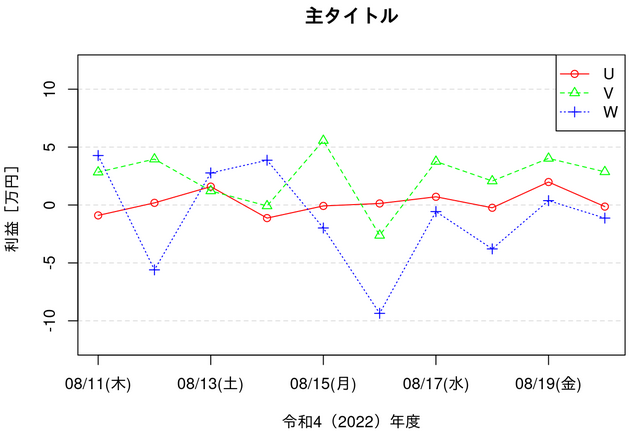
\includegraphics[width=0.5\textwidth]{timeseries_graph.png}
}
{
  時系列グラフ
}
{20}
{時系列グラフ}
{時系列図}
{time series graph}
{time series chart}

\QuizShortAnswer
{
  次のグラフを何というか?\\
  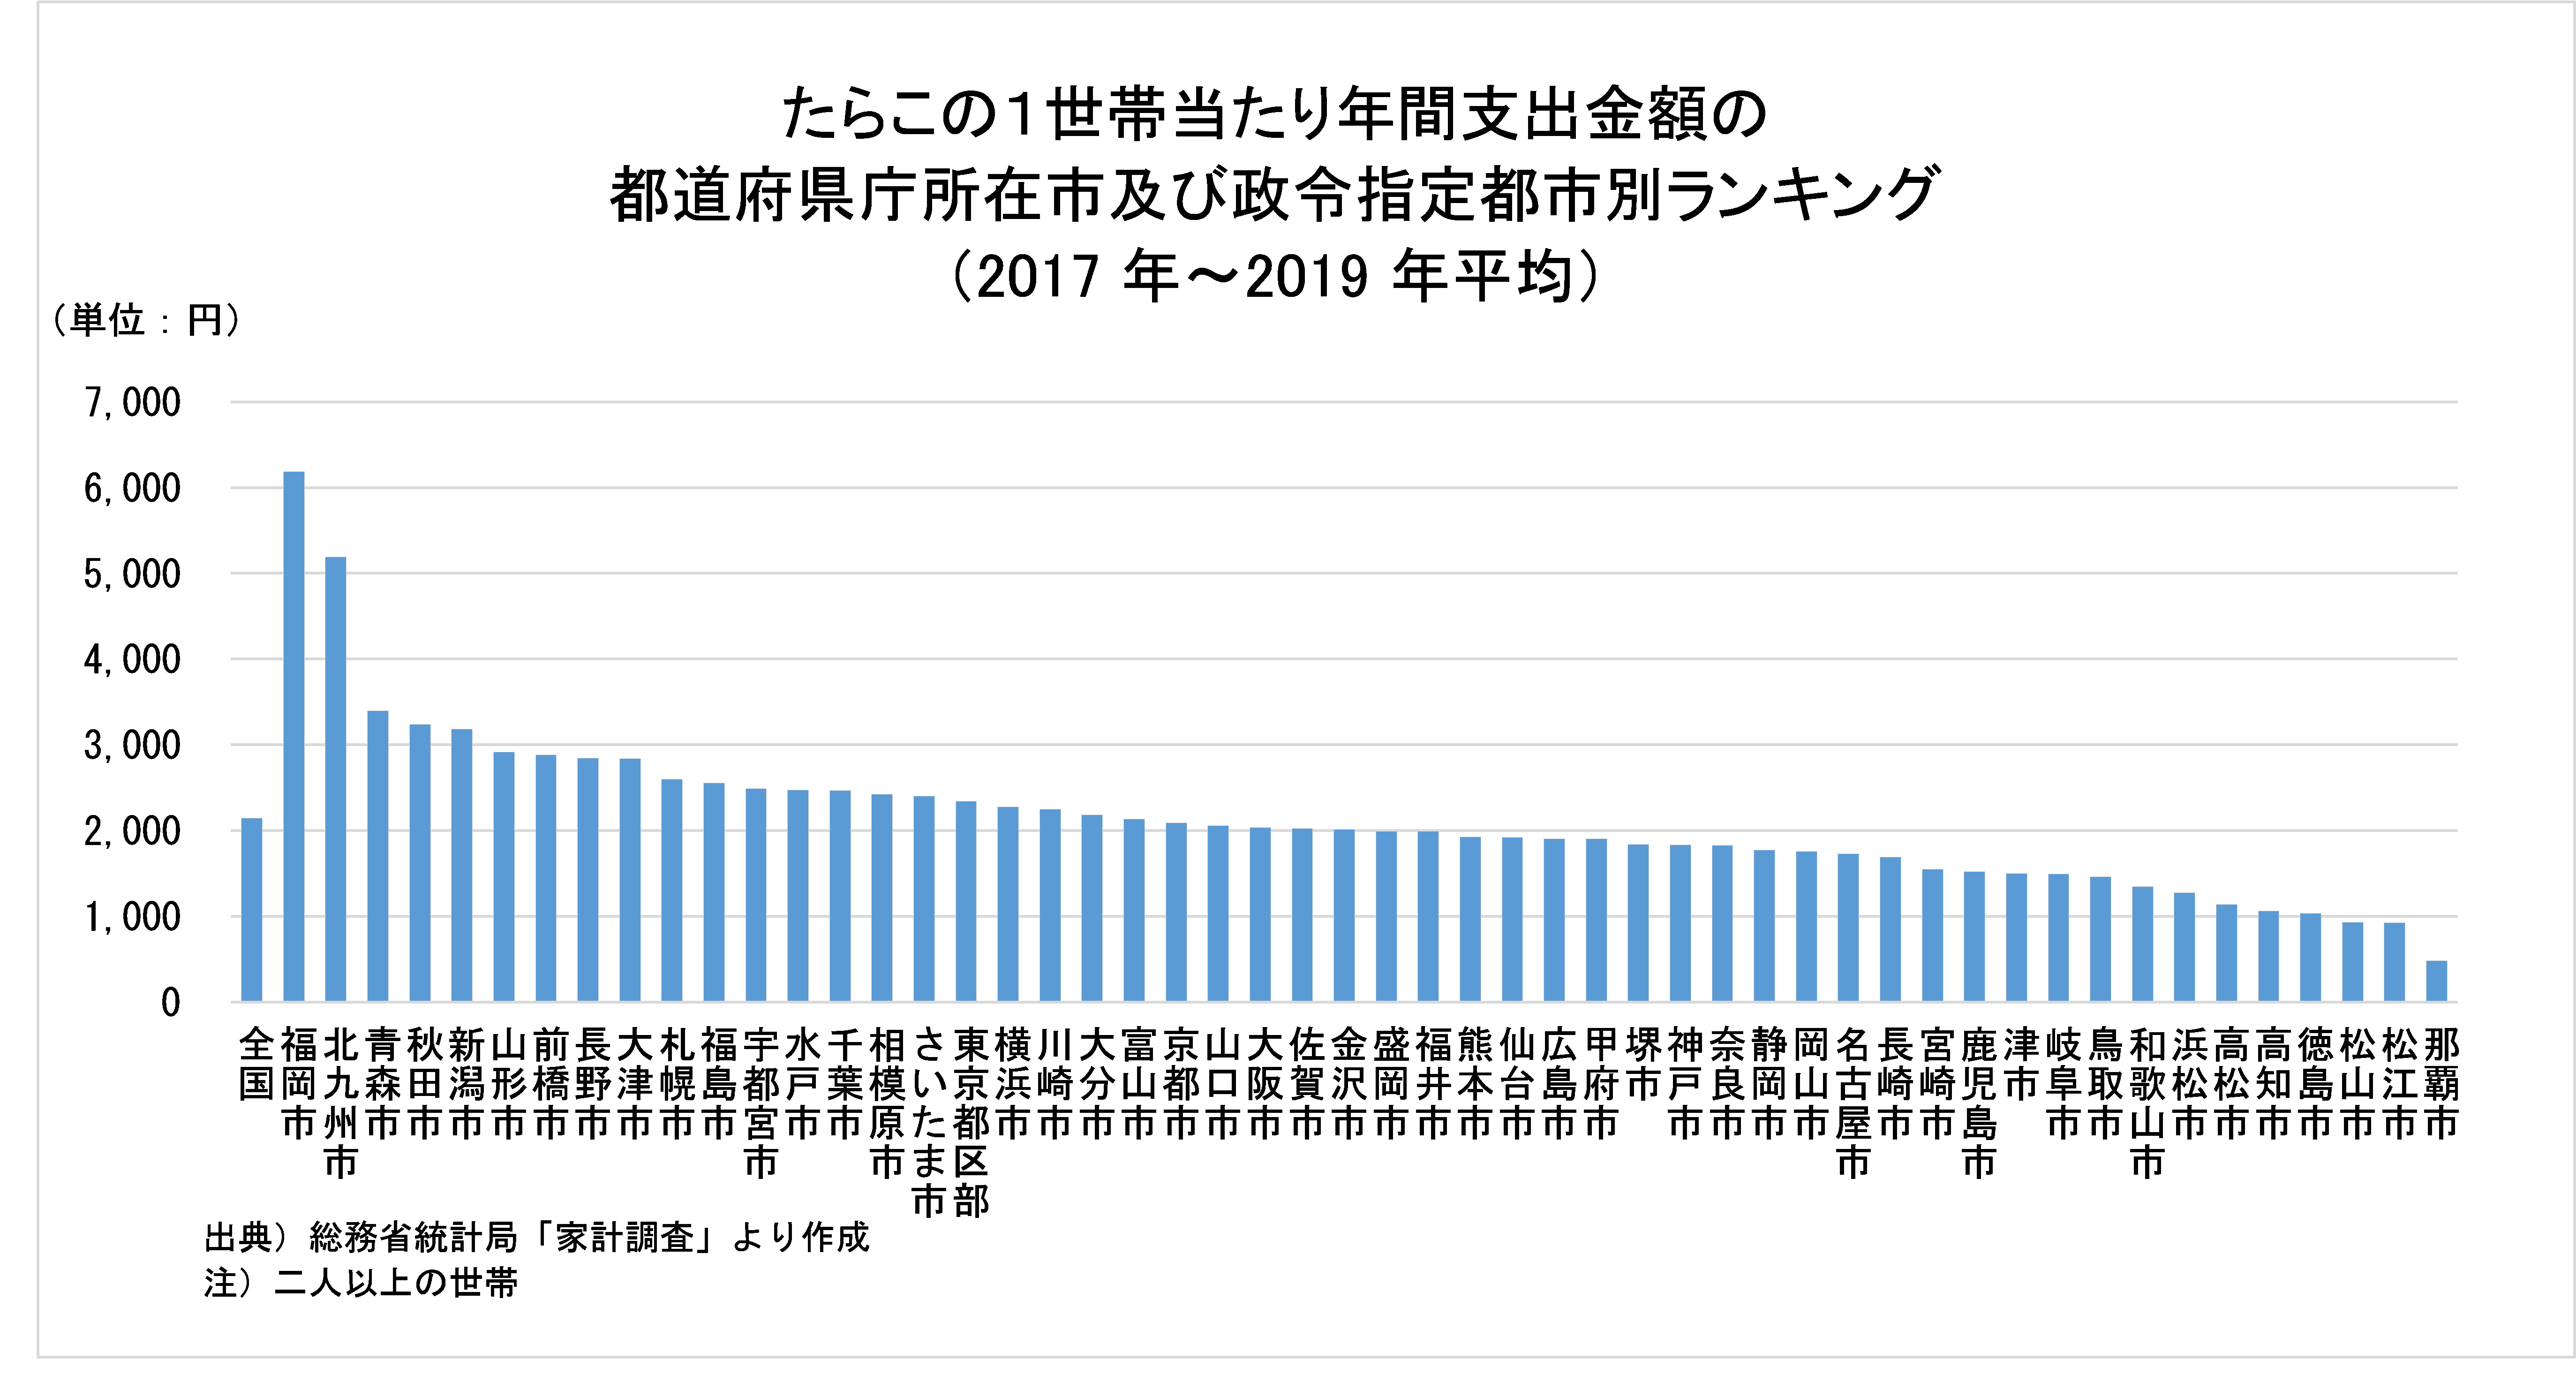
\includegraphics[width=0.5\textwidth]{barplot.png}
}
{
  棒グラフ
}
{20}
{棒グラフ}
{bar*plot}
{bar*graph}
{bar*chart}

\QuizShortAnswer
{
  次のグラフを何というか?\\
  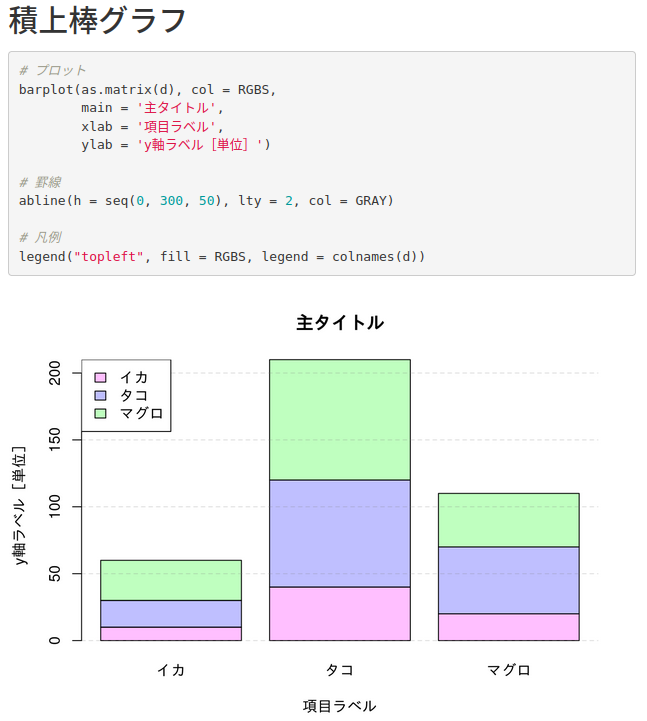
\includegraphics[width=0.5\textwidth]{barplot_graph_stacked.png}
}
{
  積上棒グラフ
}
{20}
{積*上*棒グラフ}
{stacked bar*plot}
{stacked bar*graph}
{stacked bar*chart}

\QuizShortAnswer
{
  次のグラフを何というか?\\
  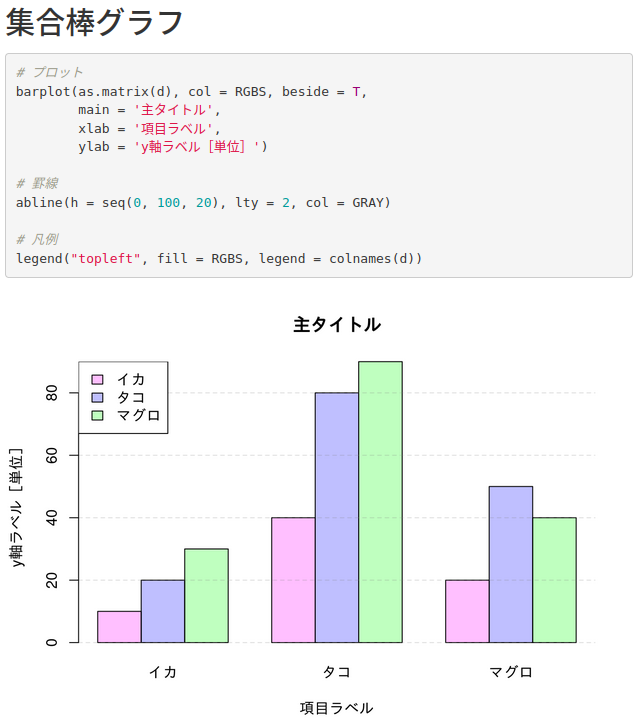
\includegraphics[width=0.5\textwidth]{barplot_graph_grouped.png}
}
{
  集合棒グラフ
}
{20}
{集合*棒グラフ}
{grouped bar*plot}
{grouped bar*graph}
{grouped bar*chart}

\end{quiz}

\end{document}
